\section{TEM}

% ~5 Bilder
% what have we seen: charging artefacts (bad sample coating/high magnification, charge buildup)

%artefakte: kleine runde Wassereinschlüsse in der Plastikbeschichtung => Loch in der Probe
%schwarze streifen: irgendwelche Fehler in der Beschichtung
%schwarze Punkte: schwere Elemente (OsO4 die ja vorher für Kontrast da reingepackt wurden).
	%OsO4 gibt Kontraste für Lipide.
	%r mehr Kontraste: Urandingens, etc. => differential staining, differential contrast (Uranylacetat??? stand iwo, aber hier Osmiumdingens)
	%robe wurde nicht richtig abgewaschen => Kristalle dieser Salze als Kontamination auf der Oberfläche
%bild mit Gitter: kondensierte dna (nucleoli,) und Helferzelle, vat-grown (also zumindest nicht aus echtem Hirn)
%dann Helferzelle.
	%hne Kontrastmittel: auf reine Eiskristalle fokussieren, dann mit der Fokussierung Zytoplasma, Mitochondrien anschauen
	%resnel-(Ränder) um die Mitochondrien durch interferenz. Nucleus ist das große Runde.
%golgi(?)-Apparatus: Zysterny, einmal senkrecht, einmal parallel geschnischnitten
%im tem ist damage durch e-beam. runde helle fläche war in voriger vergrößerung fokussiert.

In \cref{fig:tem:waben} ist eine TEM-Aufnahme bei geringer Vergrößerung zu sehen.
Deutlich sichtbar ist die Wabenstruktur des TEM-Netzes und ein Loch in der Probe. %??, das durch Wassereinschlüsse in der Plastikbeschichtung entstanden ist.

\begin{figure}[!ht]
    \centering
    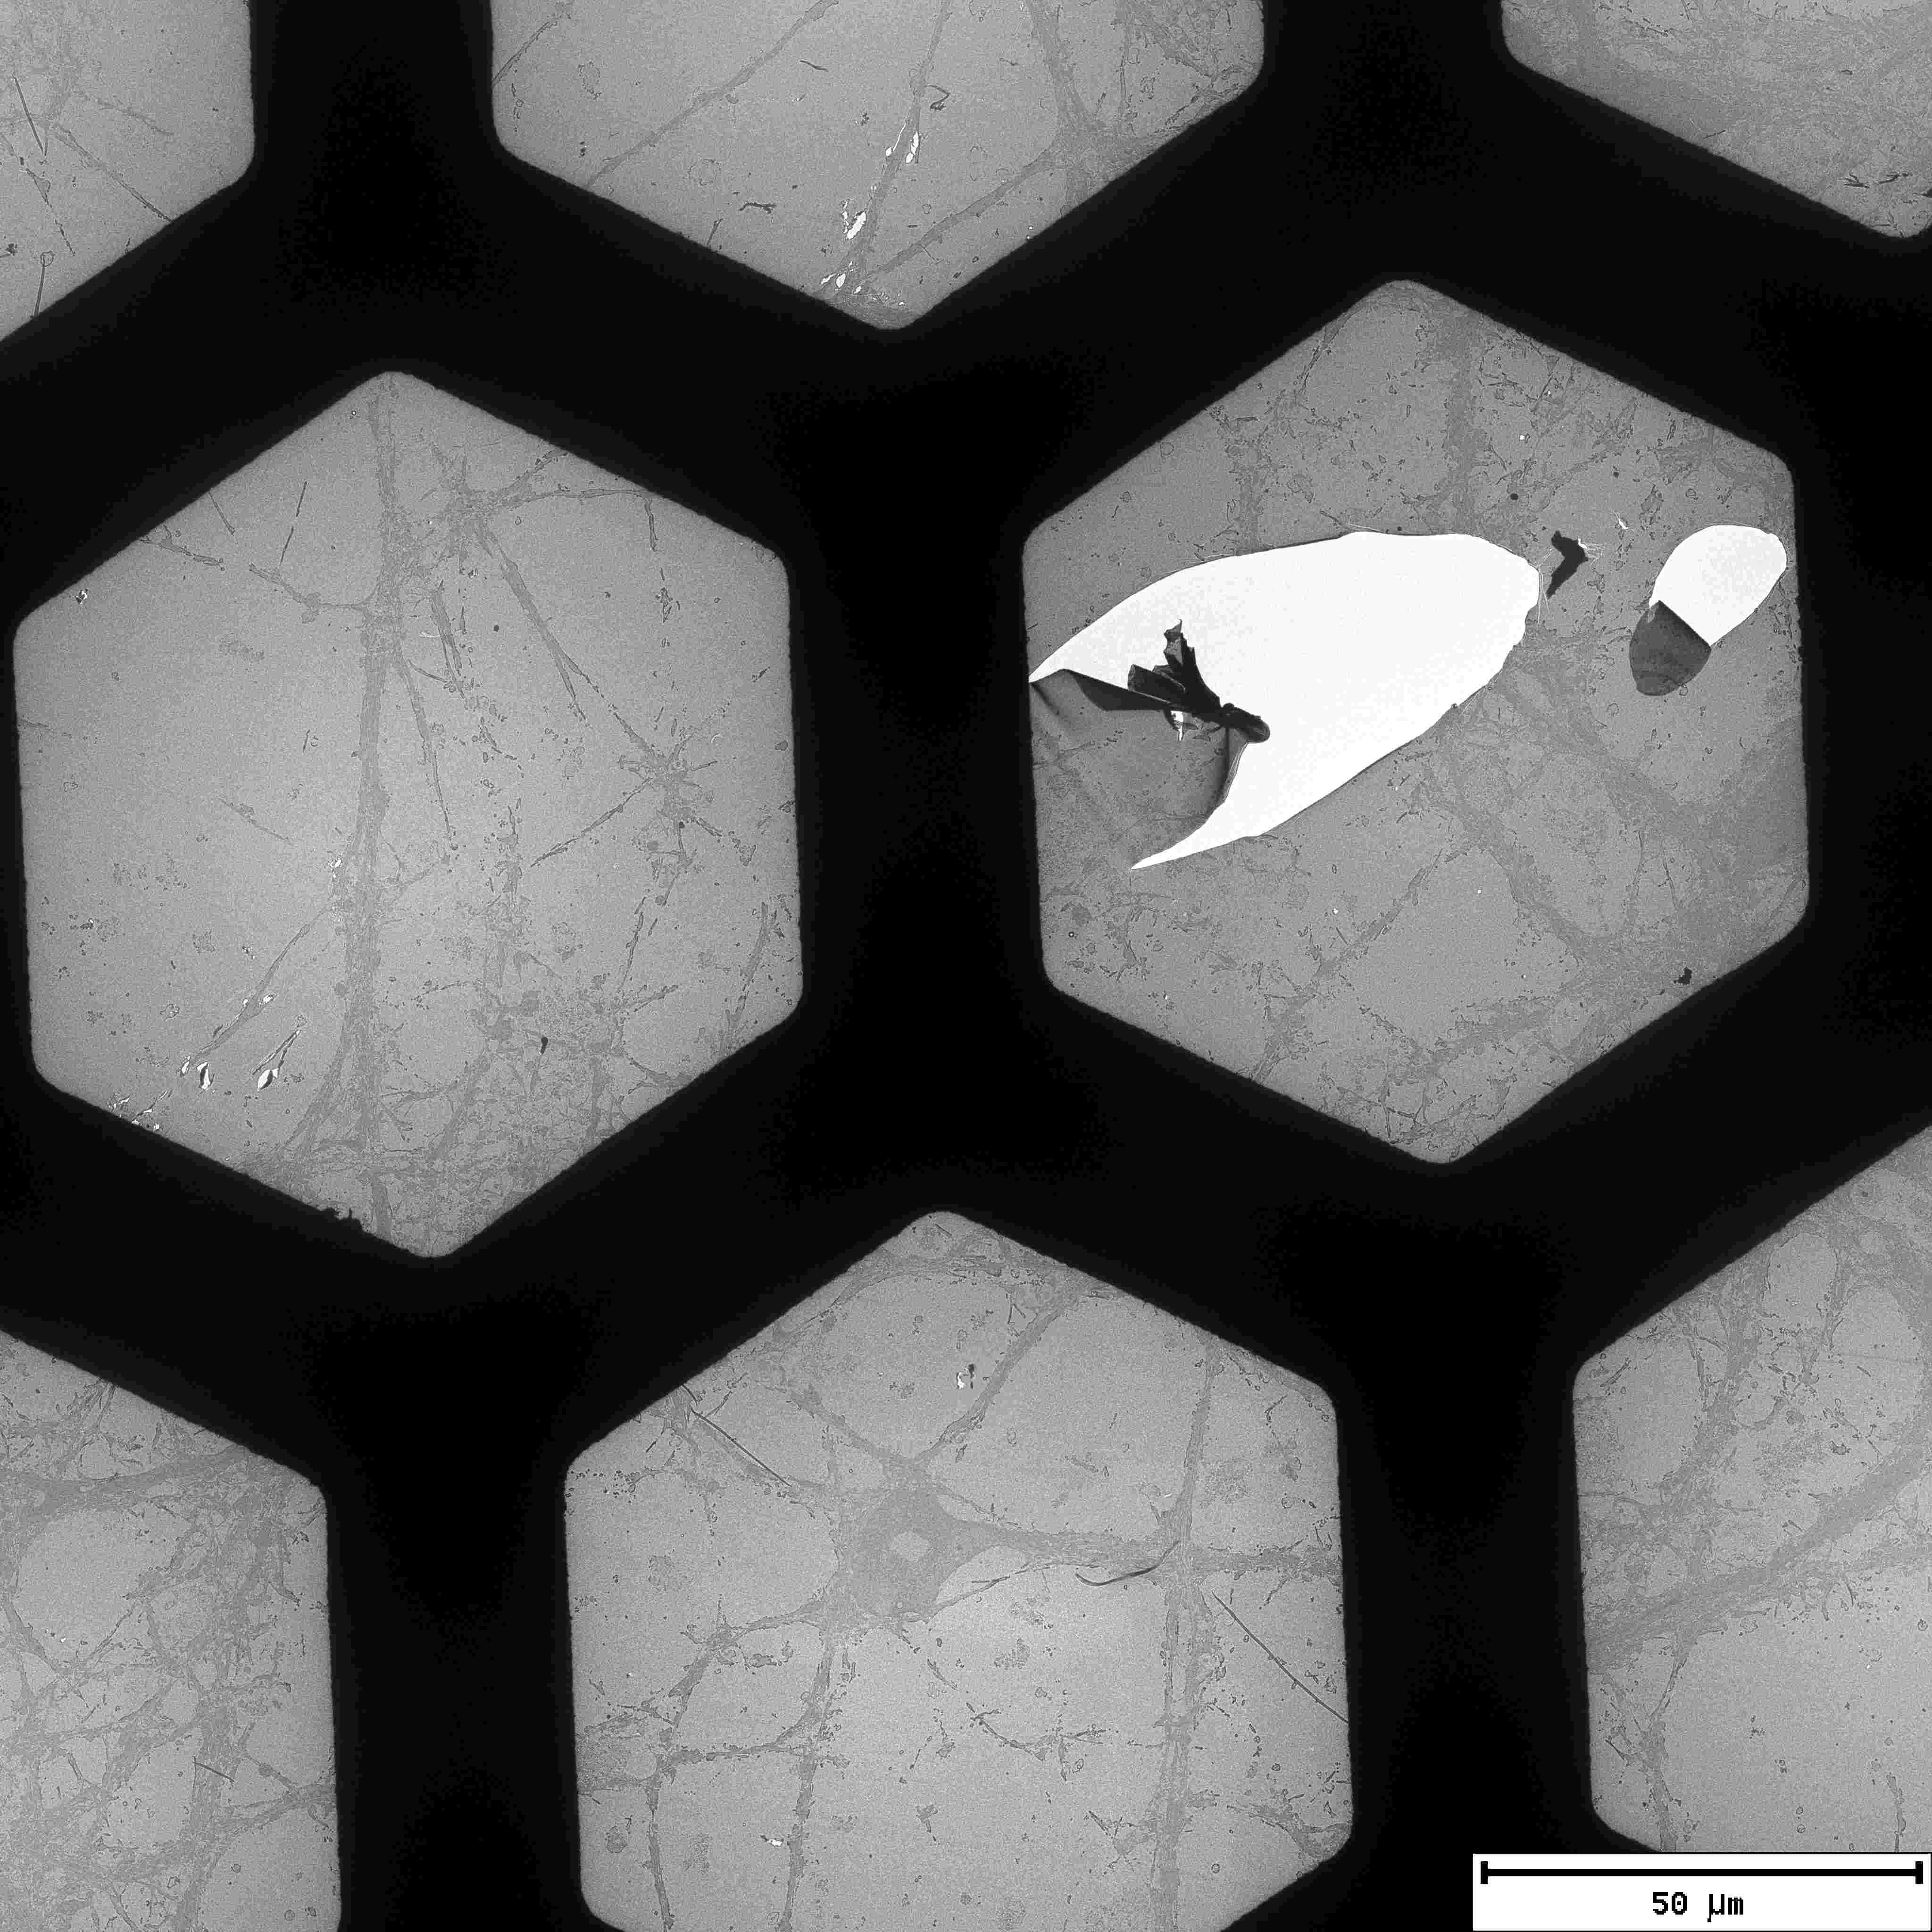
\includegraphics[width=0.65\textwidth]{img/TEM/1_low_mag_artifacts.jpg}
    \caption{TEM-Lichtbildaufnahme von kondensierter DNA (Nucleoli) und Helferzellen, in-vitro gewachsen, bei geringer Vergrößerung.}
    \label{fig:tem:waben}
\end{figure}

In \cref{fig:tem:ahk} ist die Aufnahme eines Astrozyten dargestellt.
Es sind Eiskristalle sichtbar, welche durch Fehler beim Abwaschen der Probe entstehen, wobei Salzkontaminationen auf der Oberfläche zurückgeblieben sind.
Auch hier sind Wassereinschlüsse in Form von kleinen schwarzen Punkten zu sehen.

\begin{figure}[!ht]
    \centering
    \includegraphics[width=0.65\textwidth]{img/TEM/2_astrocyte_house_keeper.jpg}
    \caption{TEM-Lichtbildaufnahme einer Astrozyten-Helferzelle im unteren linken Teil des Bildes. Fokussiert wurde auf die Eiskristalle im oberen rechten Bildbereich. Als Kontrastmittel wurde Osmium(VIII)-oxid verwendet.}
    \label{fig:tem:ahk}
\end{figure}

In \cref{fig:tem:anc} ist der Nukleus und das Zytoplasma des Astrozyten abgebildet und in \cref{fig:tem:golgi} ist der Golgi-Apparat zu sehen.
Dazu wurde zunächst auf die Eiskristalle (nicht im Bild) fokussiert, wodurch um die Mitochondrien Fresnel-Ränder (Interferenzeffekt bei Objekten vor oder hinter der Fokusebene) sichtbar werden.

\begin{figure}[!ht]
    \centering
    \includegraphics[width=0.65\textwidth]{img/TEM/2_astrocyte_nucleus_cytoplasm.jpg}
    \caption{Überfokussierte TEM-Lichtbildaufnahme von Nukleus und Zytoplasma einer Astrozyten-Helferzelle.}
    \label{fig:tem:anc}
\end{figure}

\begin{figure}[!ht]
    \centering
    \includegraphics[width=0.65\textwidth]{img/TEM/4_astrocate_Golgi.jpg}
    \caption{Überfokussierte TEM-Lichtbildaufnahme des Golgi-Apparates (Bildmitte, einmal parallel und einmal quer geschnitten) einer Astrozyten-Helferzelle. }
    \label{fig:tem:golgi}
\end{figure}


%\begin{figure}[!ht]
    %\centering
    %\includegraphics[width=0.65\textwidth]{img/TEM/5_synapse.jpg}
    %\caption{.}
    %\label{fig:tem:synapse}
%\end{figure}
%Uranylacetat war auch iwo

%Muskeln: quergestreifte Muskeln. Eine Zelle om menschl. Bizeps ist 15cm lang (Schulter bis ellenbogen), 1 Mikrometer abstand haben die schwarzen linien (Scheiben da dings)
	%ote Blutzelle oben links. bringt Glukose zu zelle, mitochondrien (Kreise) wandeln in ATP um=> Kontraktion der Mysin-Aktin-Dinger
	%chwarze Linien sind die Scheiben, wo das Aktin dranhängt und Myosin jeweils dazwischen
%irgendwas mit Platin: Platin in tiefen deposited (i think), "platinum replicas", sem-like image durch Invertierung
	%das Platin ist halt so als Form irgendwo die Topografie abgepauscht

In der Aufnahme eines Herzmuskels in \cref{fig:tem:muskel} ist die Querstreifung des Muskels deutlich zu erkennen.
Am oberen linken Bildrand ist eine rote Blutzelle sichtbar, welche Glukose zu den Muskelzellen bringt, wo die Mitochondrien (runde Strukturen) sie in ATP umwandeln und so die Kontraktion durch die Aktinfilament-Myosin-Interaktion ermöglicht.
Dabei sind die schwarzen Linien die Scheiben, an denen die Aktinfilamente hängen und dazwischen befinden sich die Myosinstränge.

\begin{figure}[!ht]
    \centering
    \includegraphics[width=0.65\textwidth]{img/TEM/9_heart_muscle.jpg}
    \caption{TEM-Lichtbildaufnahme eines Kaninchenherzmuskels}
    \label{fig:tem:muskel}
\end{figure}
